\usepackage{libertine}
\DeclareRobustCommand\textsb[1]{{\libertineSB#1}}

%\usepackage{ebgaramond}
%\usepackage{garamondlibre}
%\usepackage{CormorantGaramond}
%\usepackage{MinionPro}
\usepackage{pdfpages}
\usepackage[a-1b]{pdfx}

% below works well with hyperref, but spacing is standard (to large)
%\usepackage{sectsty}
%\sectionfont{\Large\normalfont\scshape\raggedright}
%\subsectionfont{\large\normalfont\scshape\raggedright}

  % titlesec does not play nice with RMarkdown, so hack:
\let\paragraph\oldparagraph
\let\subparagraph\oldsubparagraph
\usepackage[sc, compact, raggedright]{titlesec}
% titlesec does not play nice with hyperref, so hack:
\newcommand{\sectionbreak}{\phantomsection}
\newcommand{\subsectionbreak}{\phantomsection}
  \usepackage{titling}
\pretitle{
   \begin{minipage}{\textwidth}
   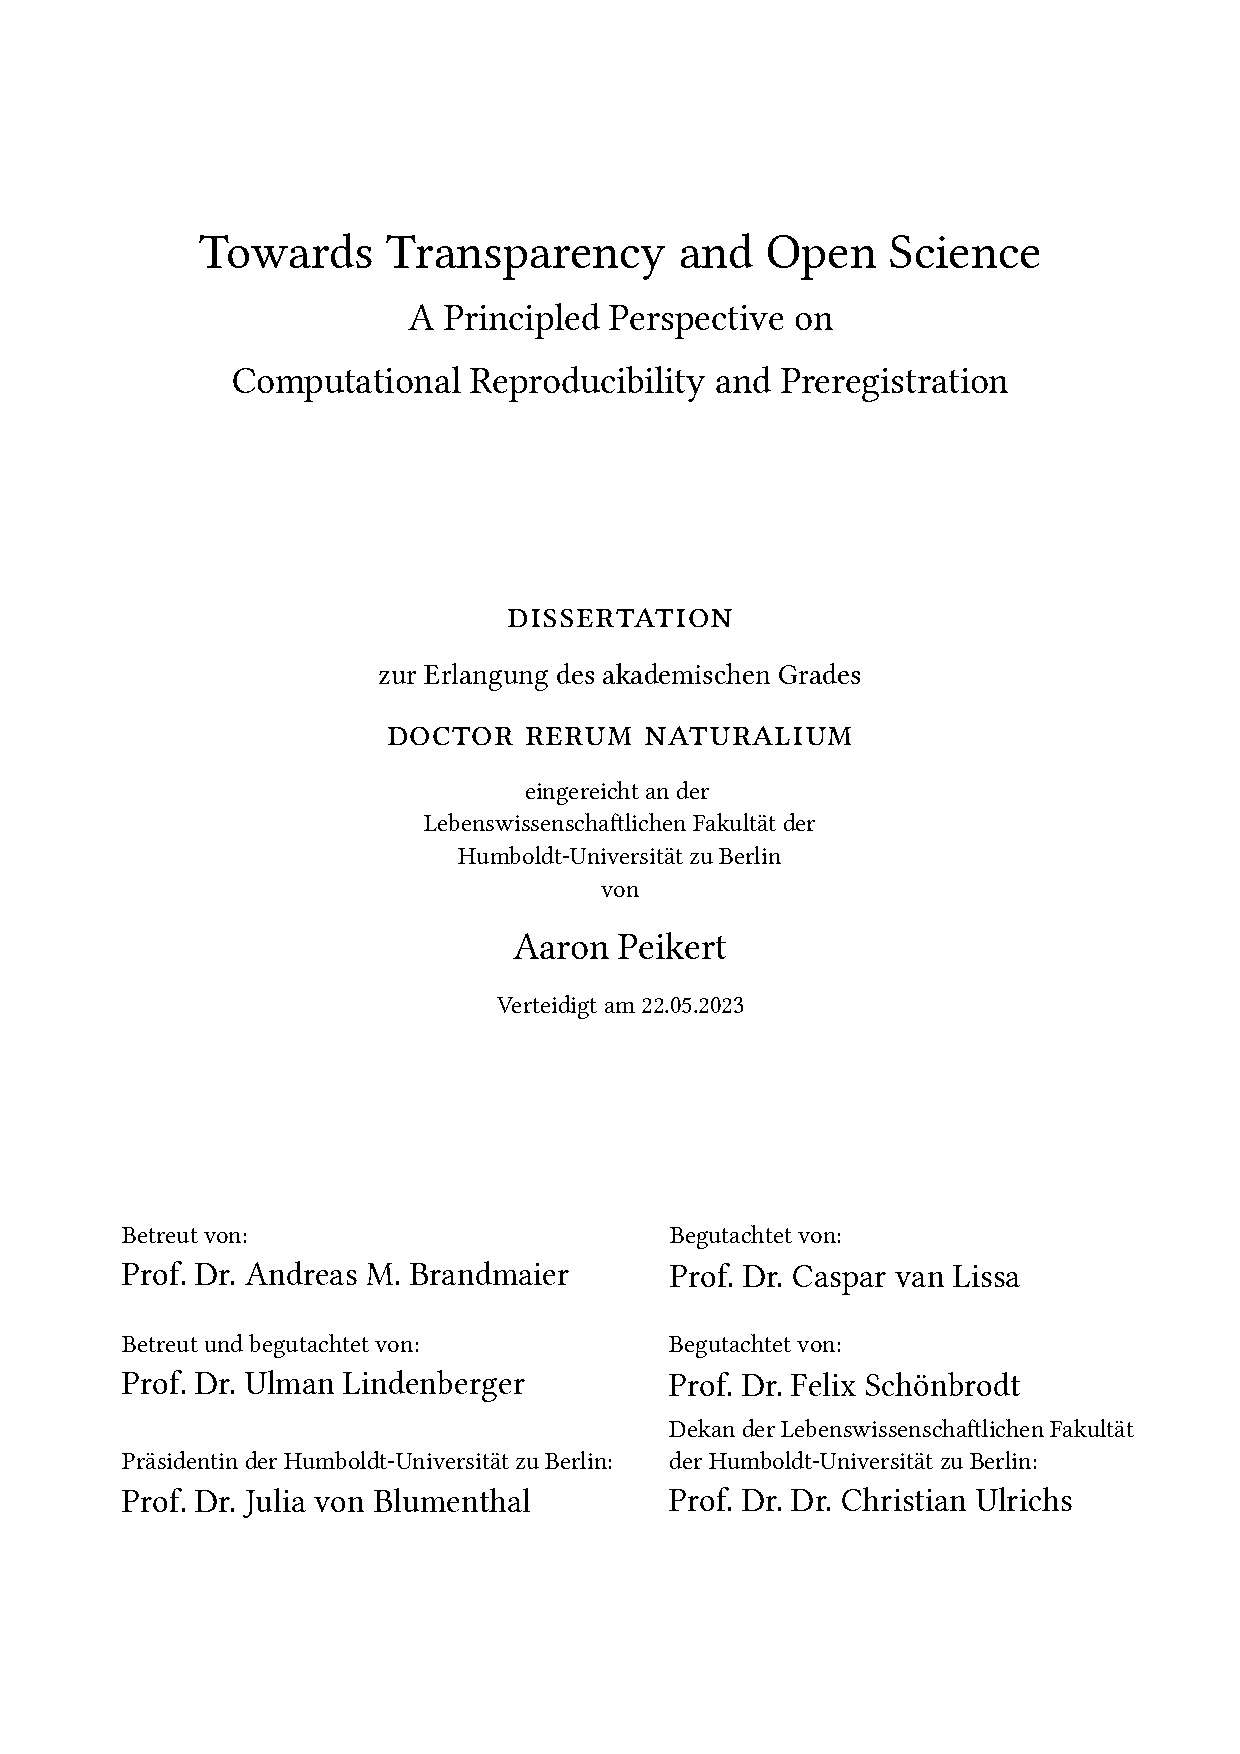
\includepdf[offset=5mm 0mm]{cover.pdf}
   \end{minipage}
   \newpage
   \clearpage%
   \thispagestyle{empty}%
   \addtocounter{page}{-2}%
   \null%
   \clearpage
   \begin{center}\LARGE}
\posttitle{\end{center}}

\usepackage{polyglossia}
\setmainlanguage[]{english}
\setotherlanguage[]{german}

\let\oldabstract\abstract
\let\oldendabstract\endabstract
\makeatletter
\renewenvironment{abstract}
{\renewenvironment{quotation}%
               {\list{}{\addtolength{\leftmargin}{-1cm} % change this value to add or remove length to the the default
                        \listparindent 1.5em%
                        \itemindent    \listparindent%
                        \rightmargin   \leftmargin%
                        \parsep        \z@ \@plus\p@}%
                \item\relax}%
               {\endlist}%
\oldabstract}
{\oldendabstract}
\makeatother
\addto{\captionsenglish}{\renewcommand{\abstractname}{\vspace{-\baselineskip}}}

\usepackage[defaultlines=2,all]{nowidow}
